%==============================================================================
\chapter{Metodologia}\label{metodologia}
%==============================================================================
Neste Capítulo é apresentado a metodologia que será adotada na realização deste trabalho, que segundo fulaninho é classificada como um pesquisa experimental, visto que esta é feita de forma controlada, ou seja, utiliza-se em ambiante apropriado, com ferramentas necessárias para a coleta de métricas.

Para a elaboração da metodologia é necessário adotar um modelo de processo de software que, de acordo com  \citeonline{SOMMERVILLE1995}, é uma representação simples de um processo de software. Cada modelo de processo surge a partir de uma perspectiva particular. Existem vários modelos de processo de software (ou paradigmas de engenharia de software) e cada modelo busca colocar ordem em uma atividade inerentemente caótica \cite{NAKAGAWA2016}. 

O modelo de processo utilizado para esse trabalho foi o Incremental. Tal modelo tem por objetivo o desenvolvimento de uma aplicação inicial, apresenta-lá as pessoas impactadas e evoluir o software ao longo do tempo, de acordo com o \textit{feedback} do usuário \cite{CAMARGO2018}. 
Na Figura \ref{fig:modelo_processo} é possível acompanhar as etapas do processo de desenvolvimento do TCC, as quais são descritas nas próximas seções.
 
\begin{figure}[!htb]
    \centering
    \caption{Processo de desenvolvimento do TCC}
    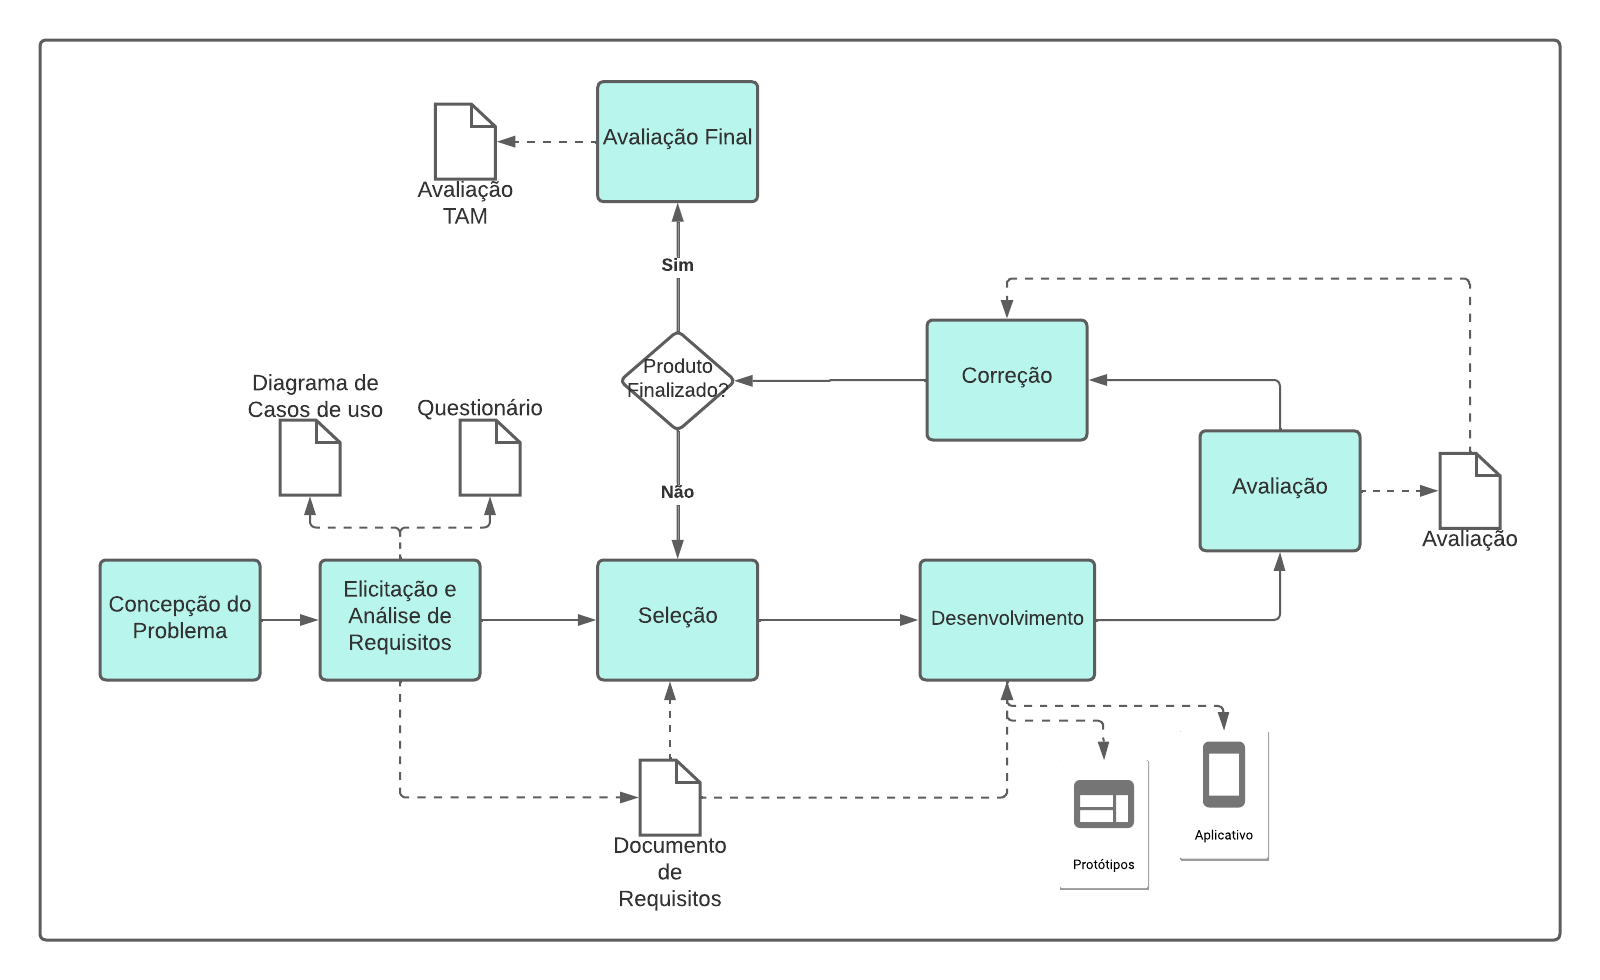
\includegraphics[width=1\textwidth]{img/metodologia.png}
    \label{fig:modelo_processo}
    Fonte - Autoria Própria
\end{figure}

\section{Concepção}
Inicialmente foi realizado uma pesquisa com o intuito de buscar trabalhos já existentes a respeito do gerenciamento de informações pessoais na área da saúde, conforme apresentado no Capítulo \ref{revisaoLiteratiraRelacionada}. A partir da análise dos estudos encontrados, foi possível definir o objetivo geral do projeto, os objetivos específicos, bem como a identificação dos \textit{stakeholders}.

%aplicação de questionário - histórias de usuário - 
\section{Engenharia de Requisitos}

Segundo \citeonline{SWEBOK2014}, Engenharia de Requisitos (E.R) é um termo muito utilizado para denominar o manejo sistemático de requisitos. Esse processo é dividido em quatro fases, a elicitação, análise, especificação e validação. A elicitação está relacionada com a origem dos requisitos. Nessa fase é necessário realizar uma coleta de fatos, onde geralmente são feitas entrevistas, questionários, reuniões e afins. Na fase da análise ocorre a elaboração dos requisitos, bem como a especificação das funções e a definição dos limites do software. Na especificação é realizada a criação de um documento que deve conter os Requisitos Funcionais (RF), Requisitos Não Funcionais (RNF) e de Qualidade. E por fim na fase de validação os requisitos podem ser validados e verificados a fim de garantir que estes tenham sido definidos sem ambiguidade e de forma compreensível para todos. 

Neste trabalho, optou-se por adotar um questionário que, de acordo com \cite{AMARO2004}, é um instrumento para coleta e análise de dados, baseando-se no que os participantes respondem nas questões direcionadas ou abertas. Para esta etapa foi elaborado um questionário, na plataforma Google Forms, sobre os cuidados com a saúde. Este apresenta questões objetivas e descritivas, sendo aberto a qualquer público acima de 18 anos. Além disso, o questionário ficou aberto por um período de 15 dias e contou com a resposta de 24 participantes. 

A partir da análise das respostas ao questionário, foi elaborado um documento de requisitos. O documento em questão serve como uma forma de comunicação entre o desenvolvedor e o usuário/cliente, com o objetivo de firmar um ``acordo'' entre as partes, com relação ao trabalho a ser desenvolvido \cite{TURINE1996}. 
Além disso, foi elaborado um diagrama de casos de uso, para modelar o comportamento do sistema, conforme a Figura. 

\textcolor{red}{diagrama de casos de uso}



%engenharia de requisitos


%A Engenharia de Requisitos (E.R) determina o processo de reconhecimento de Requisitos no qual estabelece o que deve ser feito é Elicitado, Analisado e Modelado [\cite{Leite1990} \cite{Leite1994}]. Na elicitação procura-se extrair e tornar compreensível o máximo de informações possíveis, afim de obter total conhecimento sobre o tema de interesse. Nessa fase é necessário realizar uma coleta de fatos, onde geralmente são feitas entrevistas, questionários, reuniões e afins. Já na análise de requisitos é onde acontece a especificação das funções e desempenho do sistema, bem como a definição das restrições de projeto do software \cite{PRESSMAN1994}. E por fim a modelagem que tem por objetivo a criação de modelos que descrevem estaticamente e dinamicamente o que o sistema deve fazer e como deve ser. 



%diagrama de caso de uso

%\subsection{Documento de Requisitos}
% Como resultado do processo de elicitação é criado o documento de requisitos do sistema. Este deve conter a especificação dos Requisitos Funcionais (RF), Requisitos Não Funcionais (RNF) e de Qualidade. O documento em questão serve como uma forma de comunicação entre o desenvolvedor e o usuário/cliente, com o objetivo de firmar um ``acordo'' entre as partes, com relação ao trabalho a ser desenvolvido \cite{TURINE1996}.

% Adicionalmente, esses requisitos serão priorizados, considerando as respostas do publico-alvo ao questionário.

\section{Seleção}
Nesta fase, ocorre a seleção dos requisitos a serem desenvolvidos em cada ciclo de desenvolvimento. A seleção levará em conta a prioridade de cada requisito e o tempo estimado para a sua conclusão.

\section{Desenvolvimento}
Neste etapa, os requisitos selecionados são codificados para gerar um aplicativo. Para isso, três atividades são necessárias: escolha da Tecnologia de Desenvolvimento, definição da Arquitetura de Software e criação dos Protótipos de Telas. Estas atividade são descritas a seguir. 

\subsection{Tecnologia de Desenvolvimento}
Para desenvolver aplicativos (iOS/Android) existem muitas tecnologias que auxiliam nesse processo de criação, seja com desenvolvimento híbrido ou nativo. O desenvolvimento nativo é aquele desenvolvido apenas para um sistema operacional específico. Já o desenvolvimento híbrido, é possível criar um mesmo aplicativo que poderá ser executado em qualquer sistema operacional, seja Android ou iOS. \cite{BITTENCOURT2021}. Nesta etapa é onde acontece a escolha da tecnologia que será utilizada. 

Para esta etapa, foi definida a utilização do Flutter que consiste em um \textit{framework} criado para desenvolvimento mobile e que utiliza a linguagem Dart. Com esse \textit{framework} é possível desenvolver para Android e iOS com um único código base.   


\subsection{Arquitetura de Software}
A arquitetura de software é definida como uma organização dos componentes e relacionamentos de um sistema, também pode ser considerada o pilar para qualquer projeto bem desenvolvido \cite{PINHEIRO2021}. Existem diversos tipos de arquitetura de software e sobre qual arquitetura utilizar depende de cada projeto, podendo ser combinado diferentes tipos de arquiteturas dependendo do objetivo do sistema e do problema que busca ser solucionado \cite{BALDISSERA2021}.

Na Figura \ref{fig:arquitetura_flutter} é apresentada a arquitetura do \textit{framework} FLutter.

\begin{figure}[!htb]
    \centering
    \caption{Arquitetura Flutter}
    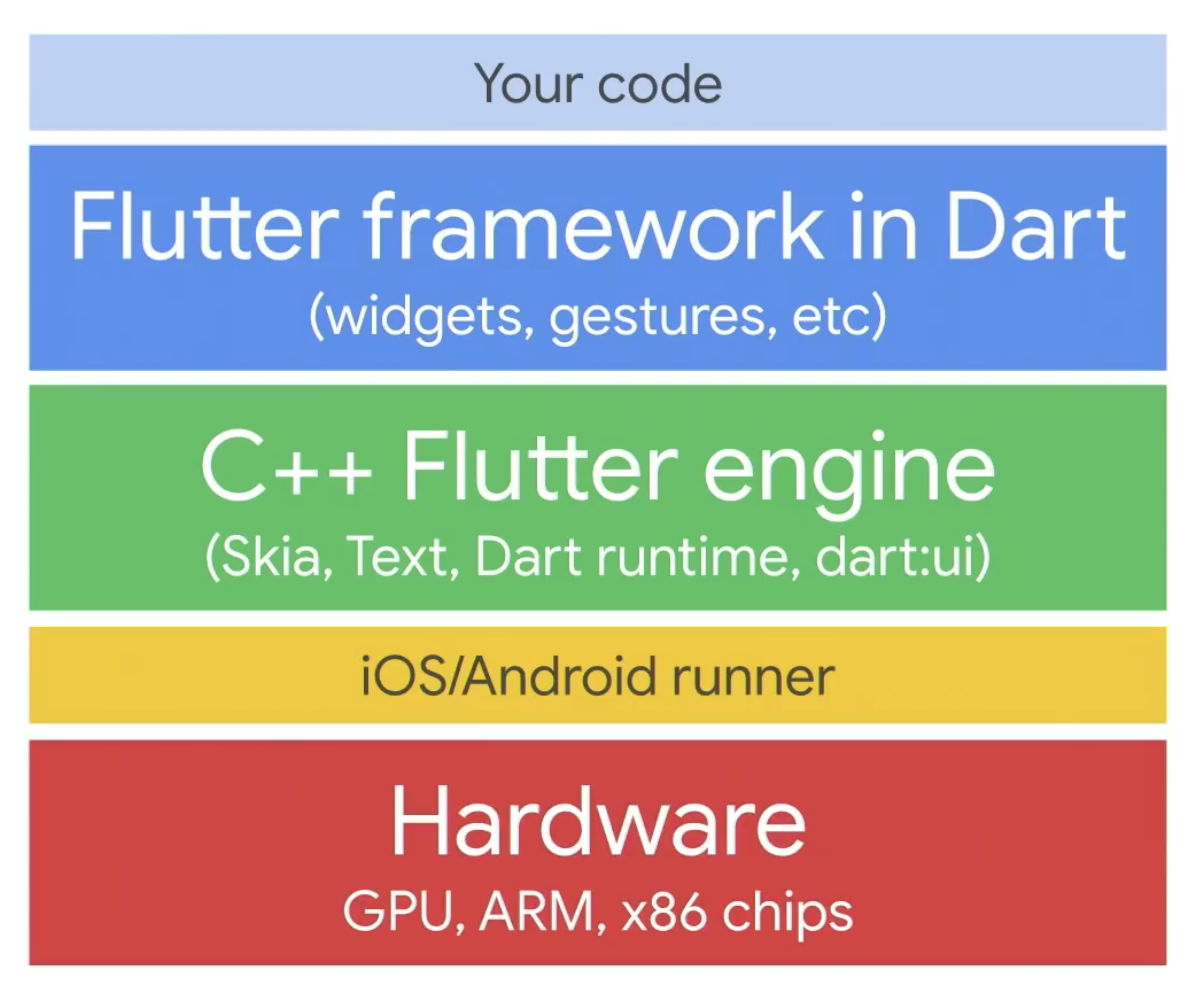
\includegraphics[width=0.6\textwidth]{img/arquitetura_flutter.png}
    \\Fonte - Site: Flutter para iniciantes 
    \label{fig:arquitetura_flutter}
\end{figure}

A camada Hardware representa a parte física do sistema. Já a camada iOS/Android \textit{runner}  é responsável por executar um código binário no Hardware. A camada Flutter \textit{engine} é responsável por gerar o código binário, composta por três bibliotecas principais: a Skia, o Text, e uma biblioteca própria do Dart para construção de interfaces. Já a camada \textit{Framework} Flutter é responsável por tudo que será renderizado na tela, desde ações mais fáceis até as mais complexas. E por fim o código do aplicativo, que fica no topo das camadas \cite{FLUTTER}.

\subsection{Prototipação de Telas}
A ideia central da prototipação é validar suas hipóteses de solução, sempre procurando envolver as pessoas impactadas (clientes/usuários) e pessoas interessadas, ou seja, desenvolvedores, gerentes de produto, etc. Uma grande vantagem da prototipação é permitir uma visão prévia do sistema final, podendo ser validada rapidamente. Nesta etapa serão desenvolvidos protótipos de alta fidelidade, utilizando a ferramenta Figma\footnote{https://www.figma.com/}, que é um editor gráfico de vetor e prototipagem de projetos de design.

\section{Avaliação}
Avaliar um software é um processo essencial para garantir que seu produto seja de qualidade para os usuários. Nesta etapa, é feita a avaliação com os \textit{stakeholders} da implementação dos requisitos selecionados para o ciclo, sob a forma de protótipos de tela ou da aplicação móvel. De acordo com as respostas dos \textit{stakeholders}, as funcionalidades em questão sofrem alguma correção ou são consideradas como ``prontas''. 

\section{Correção}
Na fase de correção, as funcionalidades que necessitam alguma alteração considerada essencial são modificadas. As demais alterações são adicionadas ao documento de requisitos e priorizadas para desenvolvimento em um ciclo futuro.

\section{Avaliação Final}
A etapa de avaliação final é realizada após o produto contemplar os requisitos essenciais para o funcionamento do aplicativo. Nesta etapa serão testadas as funcionalidades com os \textit{stakeholders}, a fim de assegurar que o software final apresente boa usabilidade, bem como confiabilidade, eficiência, manutenibilidade e portabilidade.

Para verificar se os requisitos foram desenvolvidos com sucesso será utilizado o Modelo de Aceitação de Tecnologia -\textit{Technology Acceptance Model} - (TAM). 
O TAM é capaz de medir o impacto das escolhas de design de sistemas na motivação do usuário em utilizá-los \cite{DAVIS1989}.

